We used gSound, interactive ray-tracing based sound propagation system, to perform the testing of our algorithm, and quickly realized that it is an exceptionally good example of a tool for human torture. Especially, when combined with the MS Visual Studio IDE. 

gSound \cite{schissler2011gsound} contain the following features: backward ray tracing, multi-source clustering, HRTF rendering capabilities.

Here we discuss the design (see Figure \ref{fig:figure1}) for coupling our methodology with gSound.

\begin{figure}
  \centerline{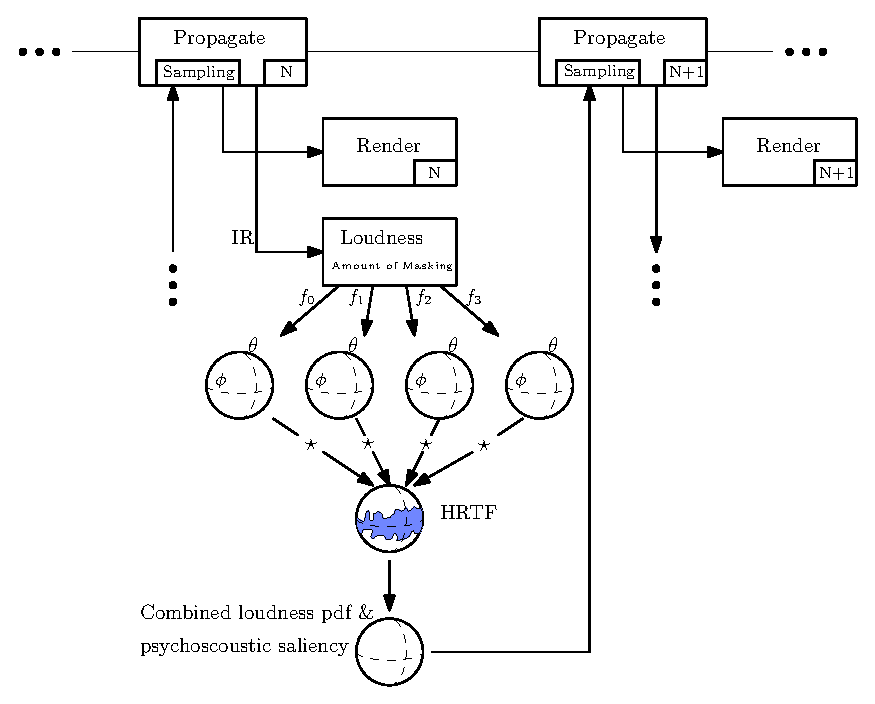
\includegraphics[width=3.0in]{figs/figure1}}
  \caption{This is a tiger.}
  \label{fig:figure1}
\end{figure}
